\documentclass[twocolumn]{article}

\usepackage{graphics}
\usepackage{graphicx}
\usepackage[utf8]{inputenc}
\usepackage{hyperref}
\usepackage{natbib}
\usepackage{hippo}

\renewcommand{\familydefault}{\sfdefault}
\newcommand{\aetitle}{External Memory Merge Sort} 
\newcommand{\studentOne}{Vincent Uhse} 

\begin{document}

\twocolumn[{\begin{small}
        \begin{minipage}{0.475 \linewidth}
          Algorithm Engineering\\
          WS 23/24
        \end{minipage}
        \begin{minipage}{0.475 \linewidth}
          \begin{flushright}
            \studentOne \\
          \end{flushright}
        \end{minipage}
      \end{small}}
    {\begin{center}
        \begin{sffamily}
          \Large\bfseries \aetitle
        \end{sffamily}
      \end{center}}
  \vskip 3em]

\begin{abstract}
    % The abstract gives a short summary of the project. Begin by stating the motivation of the research at hand, describe the problem and shortly describe what % methods you used to solve this problem. 
    % Finally, name the most important findings and provide a brief conclusion of your work.

    In this study, we compare the performance of an External Memory Merge Sort algorithm with the Classical Merge Sort algorithm,
    focusing on scenarios where data size exceeds internal memory capacity. Our motivation lies in addressing the impracticality of Classical
    Merge Sort for sorting large datasets that cannot fit into memory.

    To achieve this, we implement a block-wise data handling approach, where data is loaded into manageable blocks in internal memory. In the first phase,
    data blocks loaded, sorted and written back to external memory yielding a block-wise sorted initial partitioning. In the second phase blocks are loaded
    and merged in several merge rounds. This two-phase process characterizes External Memory Merge Sort, optimizing memory utilization and
    allowing for efficient management of massive datasets.

    Our findings reveal that External Memory Merge Sort exhibits superior performance to Classical Merge Sort for compatible data
    sizes, with larger block sizes enhancing its efficiency. We also establish that the number of merge rounds scales with an expected \( \cO\l(\log n\r) \) complexity in relation to the input
    size \( n \), while both algorithms follow a \( \cO\l(n\log(n)\r) \) time complexity trend.
    Aligning the block size with the underlying system's storage block size is relevant for optimal
    performance.

    Furthermore, our analysis suggests that run times for both algorithms do not follow a normal distribution when the input size is large, revealing
    the importance of considering statistical assumptions in algorithm performance assessment.

    In conclusion, our research highlights External Memory Merge Sort as a promising solution for efficiently sorting large datasets.
    Its adaptability, along with its superior performance under certain conditions, makes it a valuable tool in data processing applications,
    especially when internal memory limitations pose a challenge.
\end{abstract}


\section{Introduction}
% The Introduction is meant to lead the reader into the task at hand. State the motivation and purpose of your project, and name the achieved goals.

Sorting algorithms are fundamental tools extensively used in handling substantial datasets.
When tasked with sorting a substantial volume of data that exceeds the capacity of the system's internal memory, the Classical Merge Sort approach becomes impractical.
Such scenarios prompt the need for a more sophisticated solution. The External Memory Merge Sort algorithm retains the fundamental principles of Classical Merge Sort while introducing
the capability to efficiently manage files that surpass the constraints of internal memory.

In the case of External Memory Merge Sort, we employ a \(2\)-way merge (\( k = 2 \)). Both algorithms are implemented in a single-threaded fashion for this evaluation.
We compare the performance of External Memory Merge Sort against that of Classical Merge Sort.
In order to investigate various aspects of algorithm performance, we carry out a comprehensive hypothesis testing.
This includes a detailed examination of how the block size parameter impacts the efficiency of the External Memory Merge Sort.
We analyze the distribution of run times, study how the algorithms' execution times scale with larger input sizes, and assess the influence of factors such as the computing
environment and specific compiler optimization techniques on performance.

In our implementation we adopt a block-wise data handling approach. External Memory Merge Sort operates in two distinct phases.
In the initial phase, the data is organized into sorted blocks, each adhering to the designated block size.
In the second phase, the sorted blocks undergo multiple merge rounds. During each round, two small blocks are loaded from the two merge blocks into the internal memory.
These blocks are then merged to form an output block. The process continues, with small blocks reloaded as needed, and the output block written as it reaches full capacity or
at the conclusion of the merging process. This method allows us to effectively utilize approximately three times the block size within the internal memory.
We make use of only two files in external memory to keep track of unprocessed and already processed data for the current merge round.
In between two consecutive merge rounds, one file is cleared, and the other file contains blocks of sorted data, in accordance to the current block size.
In the next merge round, the filled file is read from and the empty file is written into.

We observe that External Memory Merge Sort demonstrates superior performance compared to Classical Merge Sort for compatible file sizes.
This advantage stems from the use of Quick Sort within External Memory Merge Sort for in-place sorting. Alternatively, when applying Classical Merge Sort for in-place sorting,
we observe a slightly diminished performance of External Memory Merge Sort, particularly noticeable with smaller block sizes. This discrepancy is anticipated, attributed to the
additional overhead introduced by I/O operations.
Larger block sizes generally enhance the efficiency of External Memory Merge Sort. Notably, at a fine-grained level, utilizing a block size that is a multiple of the
system's underlying storage block size leads to more efficient operation than using a size that deviates by one increment or decrement from the multiple.
This is attributed to the fact that the underlying storage block size represents the smallest loadable unit.
When the block size does not align with this multiple, some memory is loaded but remains unused, compromising algorithm efficiency.

Additionally, we determine that the number of merge rounds scales with an expected \( \cO\l(\log(n)\r) \) complexity in relation to \( n \) as the input size.
The run times for both Classical and External Memory Merge Sort scale as anticipated, following a \( \cO\l(n\log(n)\r) \) trend with \( n \) as the input size.

Furthermore, we find evidence suggesting that the run times on large data sets for both Classical and External Memory Merge Sort are unlikely to follow a normal distribution.
This observation holds true for runs on various uniform-random input files, as well as for multiple runs on the same uniform-random file.

\paragraph{}
In conclusion, our study demonstrates that External Memory Merge Sort presents a promising solution for efficiently sorting large datasets that exceed the limits of internal memory.
It outperforms Classical Merge Sort under compatible file sizes, with larger block sizes notably enhancing its efficiency.
Our findings confirm the expected logarithmic scaling of merge rounds and the anticipated \( \cO\l(n\log(n)\r) \) time complexity for both Classical and External Memory Merge Sort.
Fine-tuning the block size to align with the underlying storage block size further optimizes algorithm performance.
Additionally, the non-normal distribution of run times emphasizes the importance of considering statistical assumptions when analyzing algorithm performance.
Overall, our research underscores the effectiveness and adaptability of External Memory Merge Sort in handling substantial datasets, making it a valuable tool in data processing applications.

\section{Preliminaries}
% The preliminaries provide the reader with necessary background information. In this section the basic algorithms and the ideas behind them are explained.

\subsection{Classical Merge Sort} \label{sub:classical-explanation}
To understand the Classical Merge Sort algorithm, we begin by recognizing that lists with only one element are inherently sorted.

The process then involves doubling the chunk size by dividing the list into pairs of two.
Initially, these pairs need not be sorted. For each pair, the algorithm compares the first element with the second. If the second element is larger, they are put in the right order.
This step ensures that within each pair, the elements are sorted.
Now, we have a list of pairs, each sorted within itself. More importantly, the chunk size has doubled.

The algorithm iteratively applies this process, working on progressively larger chunks. At each step, it takes two consecutive sublists of the same size and performs a "merge" operation.
During this merge, the algorithm systematically adds elements from the two sublists into a new, larger sublist, always selecting the smaller of the two.
This merging process ensures that the sublists of a given chunk size are sorted within themselves.
After each merge round, the chunk size is doubled, leading to a progressively more sorted list until the entire original list is sorted.

\subsection{External Memory Merge Sort}
The External Memory Merge Sort algorithm efficiently sorts large datasets by employing a block-wise approach.
External Memory Merge Sort operates in two main phases.

\paragraph*{Initial Phase}
In the initial phase, the data is organized into sorted blocks, each conforming to a predefined block size that fits in the internal memory.
In this phase, we use Quick Sort to speed up the in-place sorting.

\paragraph*{Merging Phase}
The second phase involves several merge rounds where sorted blocks are merged to form larger sorted blocks. Such a merge round is visualized below (Figure \ref{fig:merge_round_diagram.pdf}).
During each merge round, two smaller blocks are loaded from the two merge sources into the internal memory.
These blocks are then merged to create an output block. As the output block reaches full capacity or at the end of the merging process, it is written to storage.
This approach uses two buffers for the input data and one output buffer. As a result, we utilize approximately three times the block size within the internal memory.
To facilitate this process, only two files in external memory are used to manage unprocessed and already processed data for the current merge round.

In between consecutive merge rounds, one file contains blocks of sorted data, partitioned according to the current block size.
The other file is cleared. In the following merge round, the filled file is read from, and the empty file is used for writing.

\section{Algorithm Engineering and Implementation}
% This section provides information about the actually used algorithms and their respective implementations. It should roughly cover the following three topics:
% Give and explain the advanced algorithms that you used, and compare them to the basic algorithms.
% Explain how you implemented these algorithms and state what external libraries you used.

\subsection{External Memory Merge Sort}
At the core of our External Memory Merge Sort implementation is the \texttt{merge\_round} function. This function processes each two consecutive sorted blocks that we
would like to merge to obtain a larger sorted block.
The two consecutive sorted blocks have length \texttt{merge\_block\_size} or less if the file has ended.
Since these blocks are too large to be held in memory at once, the function employs a strategy to handle them efficiently.

It starts by loading a small block, with a size of \texttt{block\_size} (or less if the end of the block is reached), from the first large block into memory.
Additionally, another small block of the same size (or less if the end of the block is reached) is loaded from the second large block.
These small blocks are sorted, as the larger blocks they come from are already sorted.

The goal is to merge the large blocks, but the buffer can only accommodate small blocks.
To achieve this, the function selects the smallest element from the two small blocks we have in memory and writes it into an output buffer.
It then performs an index shift to ensure that this element is not selected again. This process continues until the output buffer, which also has a size of \texttt{block\_size}, is filled.
At this point, the contents of the output buffer are written into the output file.

As elements from one of the small blocks are consumed during the merging process, the next small block from the same large block is loaded into memory to seamlessly continue the merging.
If no more blocks are available from one large block, the remaining portion of the other large block can be written directly to the output file.

Throughout this process, only small blocks and the output buffer block are held in memory, ensuring efficient memory usage.
The \texttt{merge\_round} function incrementally doubles the length of sorted blocks.
In the External Memory Merge Sort algorithm, we invoke this function repeatedly until the length of the sorted blocks reaches or exceeds the input size.
This signifies that the entire file has now been successfully sorted.

Provided below is a pseudo code representation of the \texttt{merge\_round} function (Figure \ref{fig:merge_round_pseudo_code}).
It is important to note that this is a conceptual outline of how the function operates, and for precise details and edge case behaviour, one should refer to the actual implementation.

\begin{figure*}
    \begin{center}
        \small
        \begin{lstlisting}
merge_round(char* input_file, char* output_file, input_size, merge_block_size, block_size)

// i, i_1, j, j_1 are global indices regarding the input file
// i and i_1 are used for input buffer 1
// j and j_1 are used for input buffer 2

if input_size == 0
    print information and done with method
i = 0
i_1 = min(input_size, i + block_size)
if input_size < i + merge_block_size 
    write from i to i % merge_block_size == 0 into the output, using blocks of size block_size
    making use of the output buffer, streaming blocks through the output buffer, into output file
else
    j = merge_block_size
    j_1 = min(input_size, j + block_size)

load block from i to i_1 into buffer_1
load block from j to j_1 into buffer_2

while i < i_1 and j < j_1 and k < k_1
    if buffer_1[i % block_size] < buffer_j[j % block_size]
        output_buffer[k++ % block_size] = buffer_1[i++ % block_size]
    else
        output_buffer[k++ % block_size] = buffer_2[j++ % block_size]
    if i == i_1
        write to output_buffer/to output
        if i % merge_block_size == 0
            write from j to the end of the j merge block into the output, using blocks of size block_size
            making use of the output buffer, streaming blocks through the output buffer, into output file 
        else
            load block from i to i_1 := min(input_size, i + block_size) into buffer_1
    
    if j == j_1
        if j == input_size or j % merge_block_size == 0
            write from i until the end of the i merge block into the output, using blocks of size block_size
            making use of the output buffer, streaming blocks through the output buffer, into output file 
        else
            load block from j to j_1 := min(input_size, j + block_size) into buffer_2
    
    if i % merge_block_size == 0 and j % merge_block_size == 0 and j < input_size
        i += 2 * merge_block_size
        i_1 = min(input_size, i + block_size)
        if input_size < i + merge_block_size 
            write from i to the end of the i merge block into the output, using blocks of size block_size
            making use of the output buffer, streaming blocks through the output buffer, into the output file
        else 
            j += 2 * merge_block_size
            j_1 = min(input_size, j + block_size)
\end{lstlisting}
        \normalsize
    \end{center}
    \caption{Conceptual pseudo code of the merge round function.}
    \label{fig:merge_round_pseudo_code}
\end{figure*}

A merge round is visualized in the diagram below (Figure \ref{fig:merge_round_diagram.pdf}).
\begin{figure*}
    \centering
    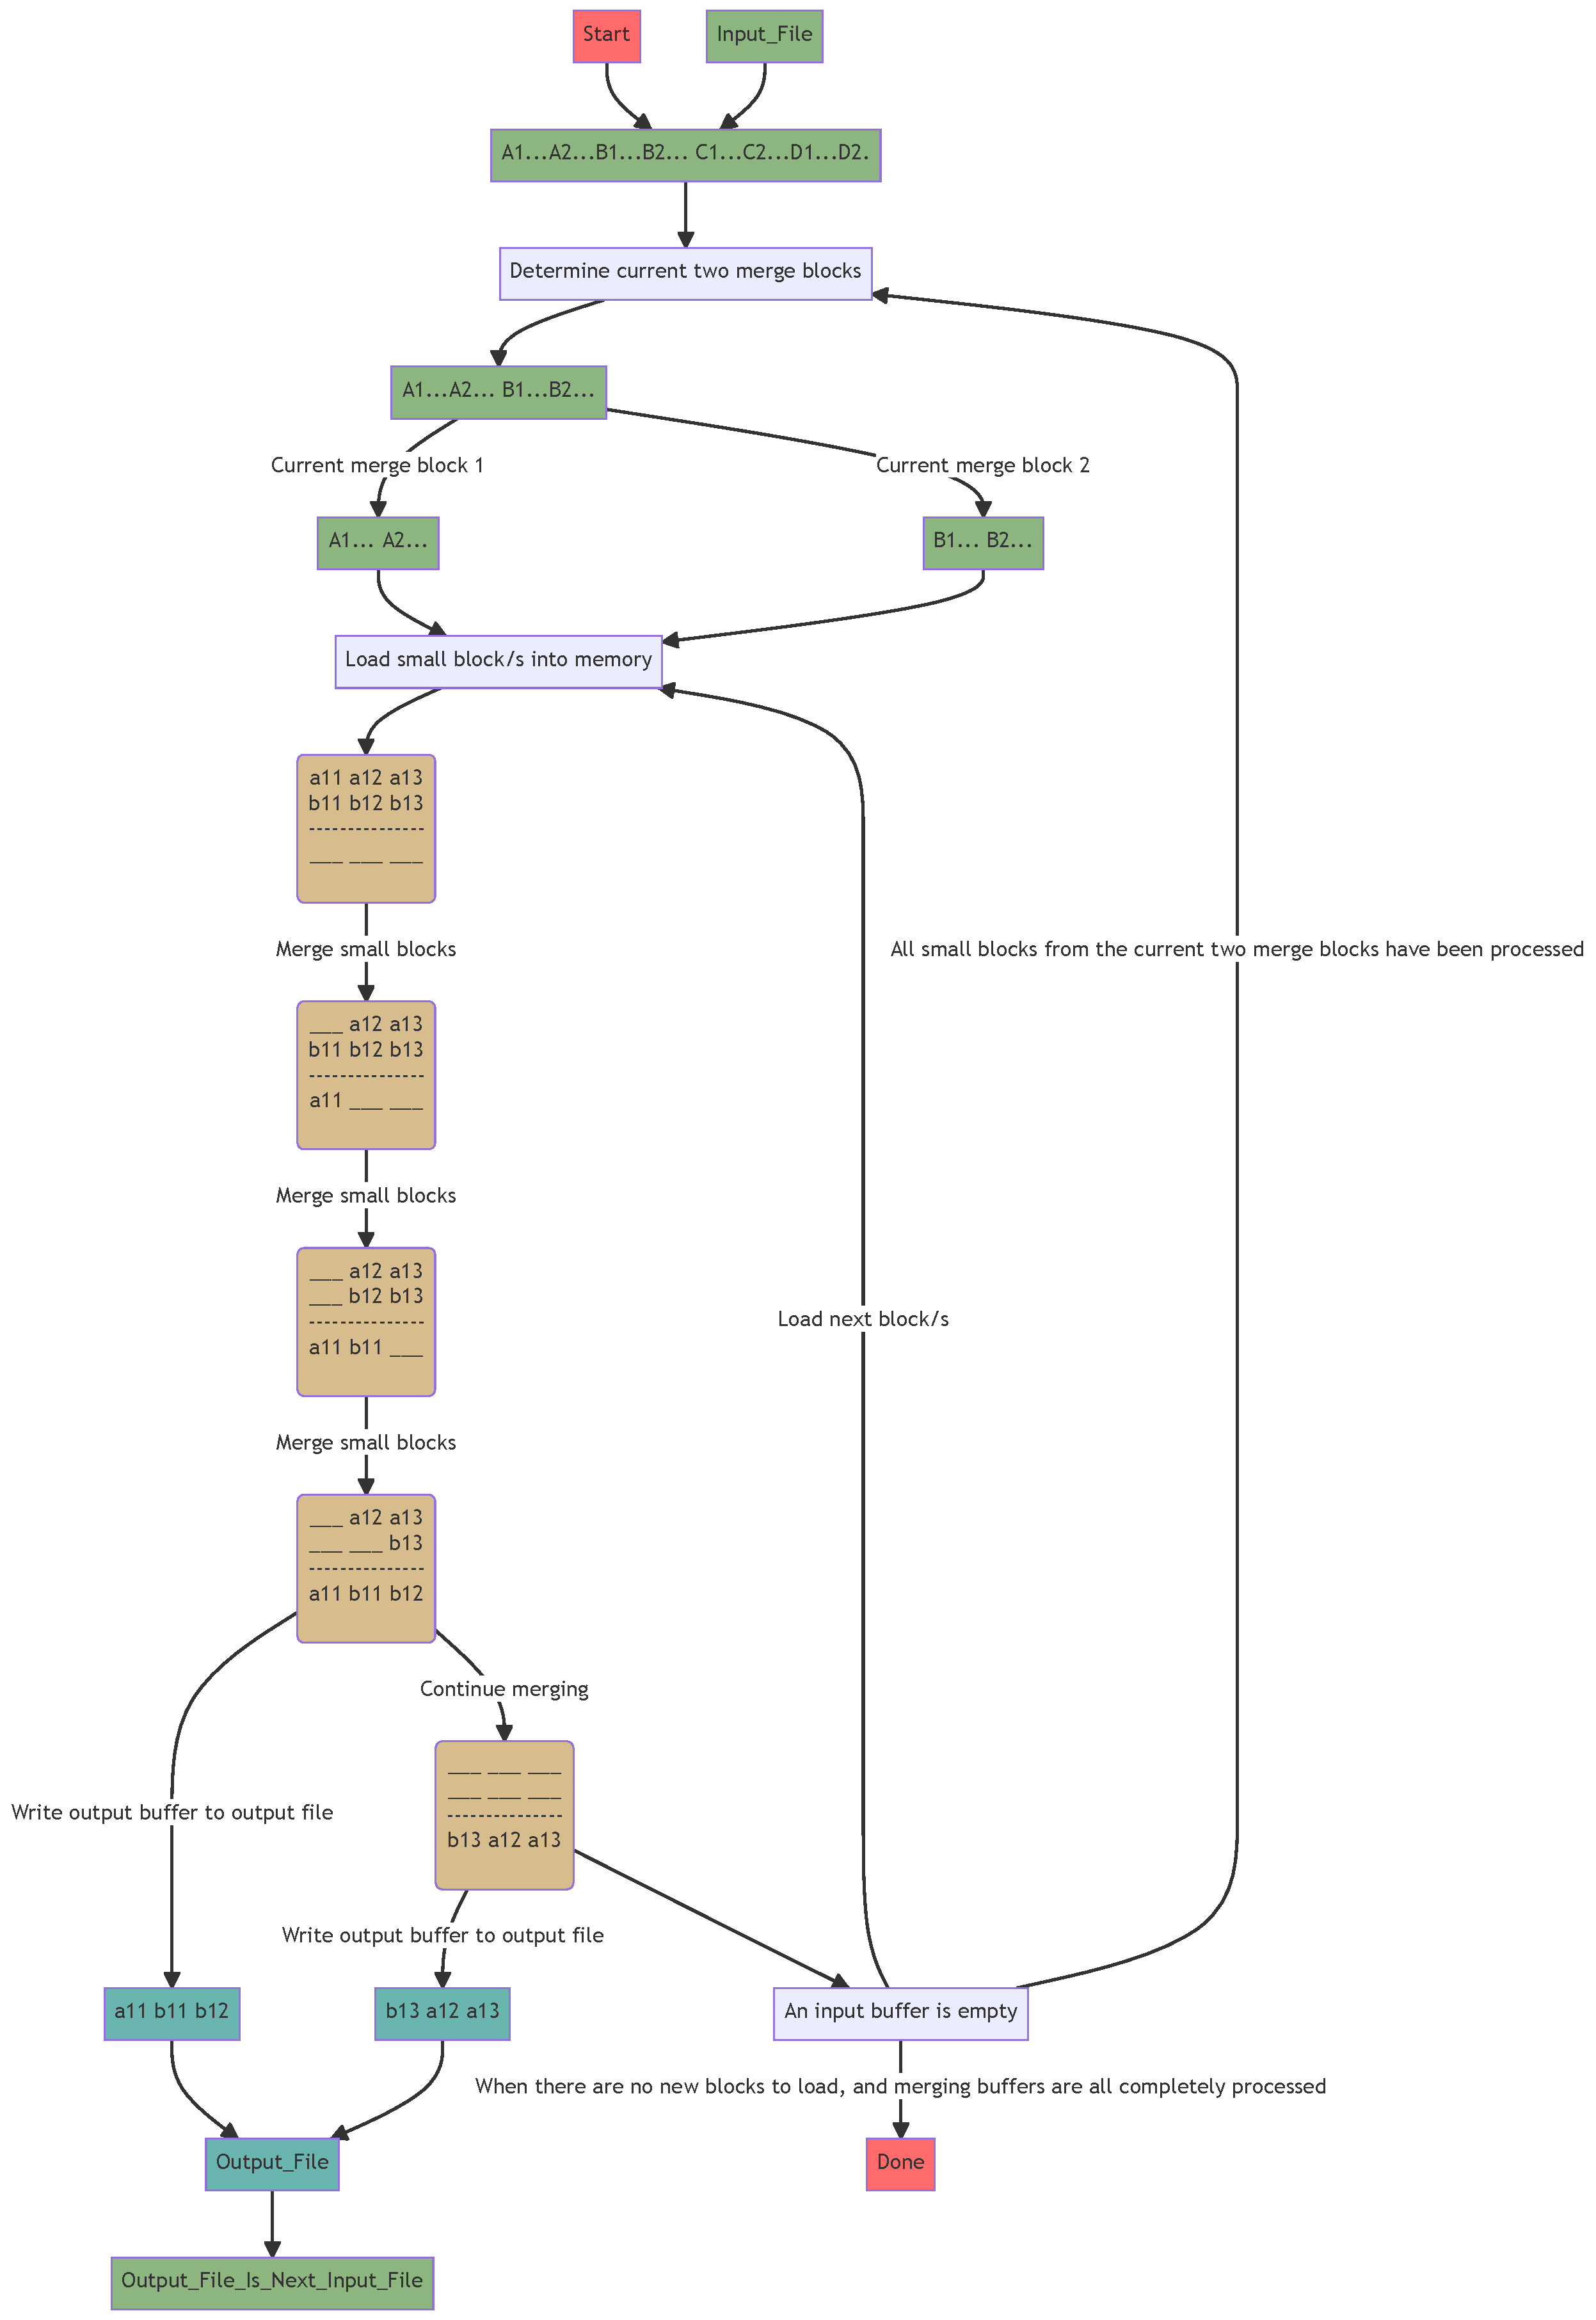
\includegraphics[width=0.9\textwidth]{./res/merge_round_diagram.pdf}
    \caption{A merge round of the External Memory Merge Sort algorithm.}
    \label{fig:merge_round_diagram.pdf}
\end{figure*}

\subsubsection*{Implementation}
To efficiently sort very large data sets, it is imperative to have precise control over system resources.
For this reason, we choose to implement the External Memory Merge Sort algorithm using the \texttt{C} programming language.
Our implementation and analysis is concerned with comparing single-threaded versions of Classical Merge Sort and External Memory Merge Sort.

\subsubsection*{Algorithm Engineering Concepts}
% State the algorithm engineering concepts that you used and explain why they were helpful (if applicable).

\paragraph*{Blocking}
We divide the data into smaller blocks that can fit into the available internal memory.
\paragraph*{Scalability}
The External Memory Merge Sort algorithm is tailored for efficiently handling exceptionally large data sets, yet it remains proficient even when processing smaller inputs.
\paragraph*{Optimal Buffer Size Selection}
We examine the influence of the block size parameter in general, as well as algorithm performance with block sizes near a multiple of the underlying system storage block size.
Selecting the block size parameter to be an exact multiple of the system storage block size yields a statistically significant, albeit small, improvement in performance.
\paragraph*{I/O Complexity Analysis}
We measure CPU time and Wall Clock time to understand in which areas our implementation has a bottleneck. Since I/O operations are generally much slower than CPU operations,
we observe that for large input sizes, the algorithm is slowed down significantly by I/O operations. This analysis lets us identify parallelism and double buffering as promising avenues for potential improvement.

\subsection{Classical Merge Sort}
If you are already familiar with how the Classical Merge Sort algorithm operates, you can proceed. Otherwise, you may refer to the explanation provided in (Subsection \ref{sub:classical-explanation}).

\section{Experimental Evaluation}
We strive to maintain strict control over the environment and adhere to a methodology that involves testing one parameter change at a time, while keeping all other variables consistent.
To enhance the robustness of our findings and mitigate potential impacts from randomness or environment-specific factors, we present experimental results across various computing environments. These results are based on repeated runs and varying random input files.

\subsection{Data and Hardware}
\label{sub:Data and Hardware}
% Here, the input data and the applied parameters are described. Further, information about the underlying hardware such as main memory and CPU is provided.

The input data is a text file containing random integers in binary format.

Computer 1 runs macOS 11.7.10 (20G1427) with 8GB internal memory and a 2.6 GHz Intel(R) Core(TM) i5-4278U processor.
Computer 2 runs an Arch Linux distribution with a kernel version 6.1.56-1-lts with 4GB internal memory and a 2.6 GHz Intel(R) Core(TM) i5-7300U  processor.
Computer 3 runs ...  % TODO
Since Computer 2 has the least internal memory, the capacity of 4GB limits the RAM size for all experiments on the different computers.

\subsection{Results}
\label{sub:Results}

\paragraph*{Analyzing the run times on four large instances}
We give the data for External Memory Merge Sort on the 0.1, 0.5, 1, 10 \( \times \) RAM size instances and for Classical Merge Sort, as this algorithm uses exclusively the internal memory, on the 0.1 and 0.5 \( \times \) RAM size instances (Table \ref{tbl:large_instances_table}).
Our configuration is based on a 4GB RAM capacity, employing a maximum block size of 1GB. This ensures that we can efficiently load up to three blocks into the internal memory, accommodating even the computer with the most limited available internal memory.
We opted not to use a block size equivalent to one-third of the available RAM size. Although technically feasible, we noticed a decrease in performance compared to the 1GB solution. This was attributed to an increase in swapping activity, which adversely affected execution speed.
\begin{figure}[htb]
    \begin{minipage}{0.475\textwidth}
        \begin{tabularx}{\textwidth}{|X|S[table-format=2.2]|S[table-format=3.2]|S[table-format=3.2]|S[table-format=4.2]|}
            \hline
                   & \multicolumn{4}{c|}{Input Size / RAM Size}                             \\ \hline
                   & 0.1                                        & 0.5    & 1      & 10      \\ \hline
            C1 (E) & 19.44                                      & 106.08 & 253.94 & 3870.50 \\ \hline
            C1 (C) & 36.63                                      & 193.94 &        &         \\ \hline
            C2 (E) & 22.07                                      & 111.52 & 368.62 & 7828.52 \\ \hline
            C2 (C) & 20.35                                      & 191.25 &        &         \\ \hline
            C3 (E) &                                            &        &        &         \\ \hline % TODO
            C3 (C) &                                            &        &        &         \\ \hline % TODO
        \end{tabularx}
        \captionof{table}{Algorithm performance comparison on large instances of External Memory Merge Sort versus Classical Merge Sort with run times in seconds rounded to two decimal places.
            In our naming scheme, "C1 (E)" represents the execution of the External Memory Merge Sort algorithm on Computer 1.}
        \label{tbl:large_instances_table}
    \end{minipage}
\end{figure}

\paragraph*{Analyzing the scaling of the algorithms' time complexity}
We bolster the theoretical assumption that run times should exhibit a \( \mathcal{O} (n \log n) \) scaling pattern using real-world experimental data.
We calculate correlation coefficients for functions representing different run time complexities. This enables us to discern the most robust linear relationship.
For the External Memory Merge Sort algorithm run times we find nearly perfect correlation, suggesting a precise linear relationship (Figure \ref{fig:Correlation_External_Wall_Clock_Time.pdf}).
For the Classical Merge Sort algorithm run times we have the same finding with a \( \Theta(n \log n) \) run time complexity (Figure \ref{fig:Correlation_Classical_Wall_Clock_Time.pdf}).
The number of merge rounds scale with \( \Theta (\log n) \) which is expected (Figures \ref{fig:Correlation_Merge_Rounds.pdf} and \ref{fig:Correlation_Classical_Rounds.pdf}).
The best fitting function for the merge rounds in the External algorithm deviates from our initial expectations. This discrepancy is due to the fact that, with the utilization of larger block sizes, the number of merge rounds is low, and here in the range of \( 0, 1, 2 \) (Figure \ref{fig:Correlation_Merge_Rounds.pdf}).

\begin{figure}[htb]
    \begin{minipage}{0.475 \textwidth}
        \centering
        \includegraphics[width=\textwidth]{./res/fit/Correlation_External_Wall_Clock_Time.pdf}
        \caption{Correlation coefficients over powers \( p \) of measured External algorithm run times with functions \( n \mapsto n^p \log n\). The curves are split by the block size parameter used in the External Memory Merge Sort algorithm.}
        \label{fig:Correlation_External_Wall_Clock_Time.pdf}
    \end{minipage}
\end{figure}

\begin{figure}[htb]
    \begin{minipage}{0.475 \textwidth}
        \centering
        \includegraphics[width=\textwidth]{./res/fit/Correlation_External_Wall_Clock_Time.pdf}
        \caption{Correlation coefficients over powers \( p \) of measured Classical algorithm run times with functions \( n \mapsto n^p \log n\).}
        \label{fig:Correlation_Classical_Wall_Clock_Time.pdf}
    \end{minipage}
\end{figure}

\begin{figure}[htb]
    \begin{minipage}{0.475 \textwidth}
        \centering
        \includegraphics[width=\textwidth]{./res/fit/Correlation_Merge_Rounds.pdf}
        \caption{Correlation coefficients over powers \( p \) of measured External algorithm merge rounds with functions \( n \mapsto n^p \log n\). The curves are split by the block size parameter used in the External Memory Merge Sort algorithm.}
        \label{fig:Correlation_Merge_Rounds.pdf}
    \end{minipage}
\end{figure}

\begin{figure}[htb]
    \begin{minipage}{0.475 \textwidth}
        \centering
        \includegraphics[width=\textwidth]{./res/fit/Correlation_Classical_Rounds.pdf}
        \caption{Correlation coefficients over powers \( p \) of measured Classical algorithm merge rounds with functions \( n \mapsto n^p \log n\).}
        \label{fig:Correlation_Classical_Rounds.pdf}
    \end{minipage}
\end{figure}

Following this, we generate visualizations of the correlation coefficients, facilitating the identification of the best-fitting function.
In addition, we conduct regression analyses to develop regression models for each of the functions.
This yields visual representations of both the \( R^2 \) values and the residuals of the fits. The data from the \( R^2 \) values match the patterns from the correlation analysis and provide no further insight into the most suitable fitting function, so they are not shown here.
To enhance our grasp of the relationship between regression residuals and the best fitting function, it is important to observe that the residuals most tightly clustered around zero are associated with the best fitting function (along with other desirable criteria like homoscedasticity and normality)
(Figures \ref{fig:kde_residuals_Correlation_External_Wall_Clock_Time.pdf},
\ref{fig:kde_residuals_Correlation_Classical_Wall_Clock_Time.pdf},
\ref{fig:kde_residuals_Correlation_Merge_Rounds.pdf} and
\ref{fig:kde_residuals_Correlation_Classical_Rounds.pdf}
).

\begin{figure}[htb]
    \begin{minipage}{0.475 \textwidth}
        \centering
        \includegraphics[width=\textwidth]{./res/fit/kde_residuals_Correlation_External_Wall_Clock_Time.pdf}
        \caption{Kernel density estimation of residuals for regression analyses with different model functions fit into run times of the External algorithm.}
        \label{fig:kde_residuals_Correlation_External_Wall_Clock_Time.pdf}
    \end{minipage}
\end{figure}

\begin{figure}[htb]
    \begin{minipage}{0.475 \textwidth}
        \centering
        \includegraphics[width=\textwidth]{./res/fit/kde_residuals_Correlation_External_Wall_Clock_Time.pdf}
        \caption{Kernel density estimation of residuals for regression analyses with different model functions fit into run times of the Classical algorithm.}
        \label{fig:kde_residuals_Correlation_Classical_Wall_Clock_Time.pdf}
    \end{minipage}
\end{figure}

\begin{figure}[htb]
    \begin{minipage}{0.475 \textwidth}
        \centering
        \includegraphics[width=\textwidth]{./res/fit/kde_residuals_Correlation_Merge_Rounds.pdf}
        \caption{Kernel density estimation of residuals for regression analyses with different model functions fit into merge rounds of the External algorithm.}
        \label{fig:kde_residuals_Correlation_Merge_Rounds.pdf}
    \end{minipage}
\end{figure}

\begin{figure}[htb]
    \begin{minipage}{0.475 \textwidth}
        \centering
        \includegraphics[width=\textwidth]{./res/fit/kde_residuals_Correlation_Classical_Rounds.pdf}
        \caption{Kernel density estimation of residuals for regression analyses with different model functions fit into merge rounds of the Classical algorithm. We observe an exception due to very small numbers of merge rounds for the largest block size.}
        \label{fig:kde_residuals_Correlation_Classical_Rounds.pdf}
    \end{minipage}
\end{figure}

\paragraph*{Analyzing Distributions of Run Times as the Input Size Grows}
We observe a shift towards normality of run times from repeated runs on fixed input files as the data sets get large and in relation to a fixed block size (Figure \ref{fig:plot_normality.pdf}).
For the distribution of run times over various input files for a fixed input size, we reject similarity with a normal distribution type.

\begin{figure}[htb]
    \begin{minipage}{0.475 \textwidth}
        \centering
        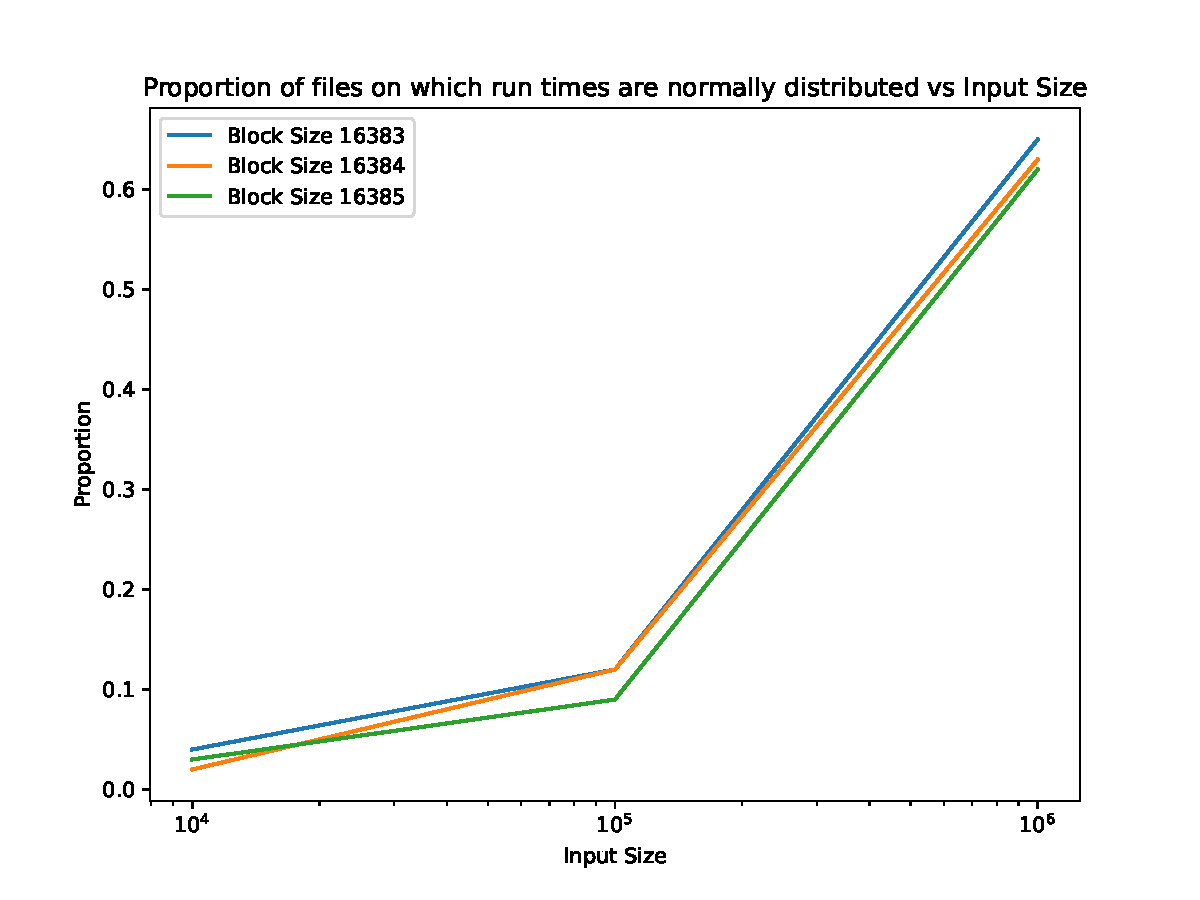
\includegraphics[width=\textwidth]{./res/plot_normality.pdf}
        \caption{}
        \label{fig:plot_normality.pdf}
    \end{minipage}
\end{figure}

\paragraph*{Analyzing I/O Overhead as the Input Size Increases}
The proportion of total run time vs CPU run time increases as the input size gets large. This is due to waiting for I/O operations to complete and shown in Figures
\ref{fig:overhead.pdf} and \ref{fig:overhead_ratio.pdf}.

\begin{figure}[htb]
    \begin{minipage}{0.475 \textwidth}
        \centering
        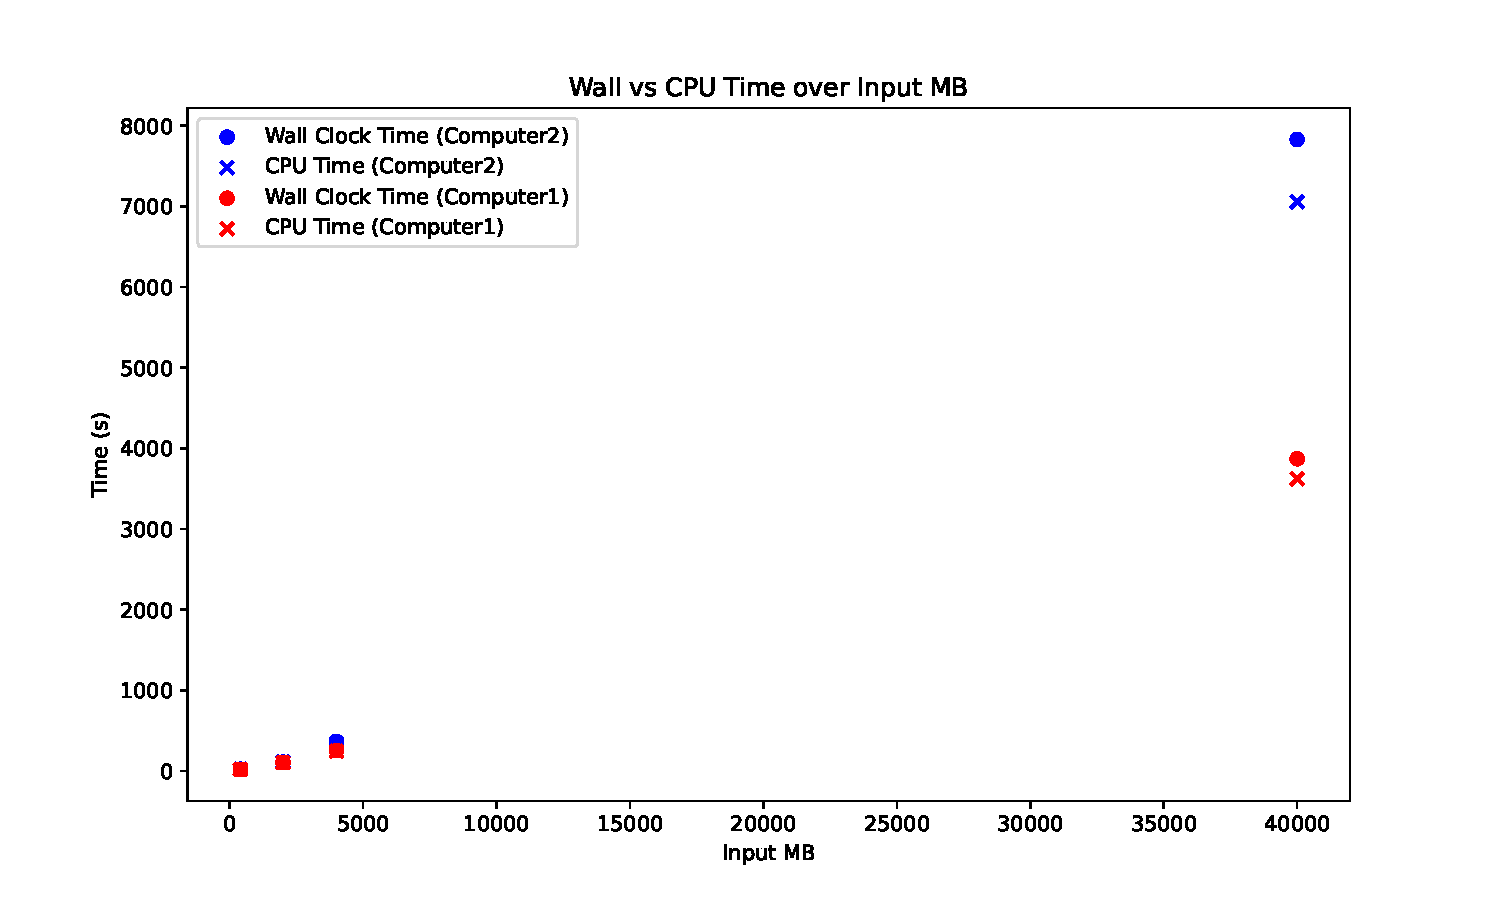
\includegraphics[width=\textwidth]{./res/overhead.pdf}
        \caption{}
        \label{fig:overhead.pdf}
    \end{minipage}
\end{figure}

\begin{figure}[htb]
    \begin{minipage}{0.475 \textwidth}
        \centering
        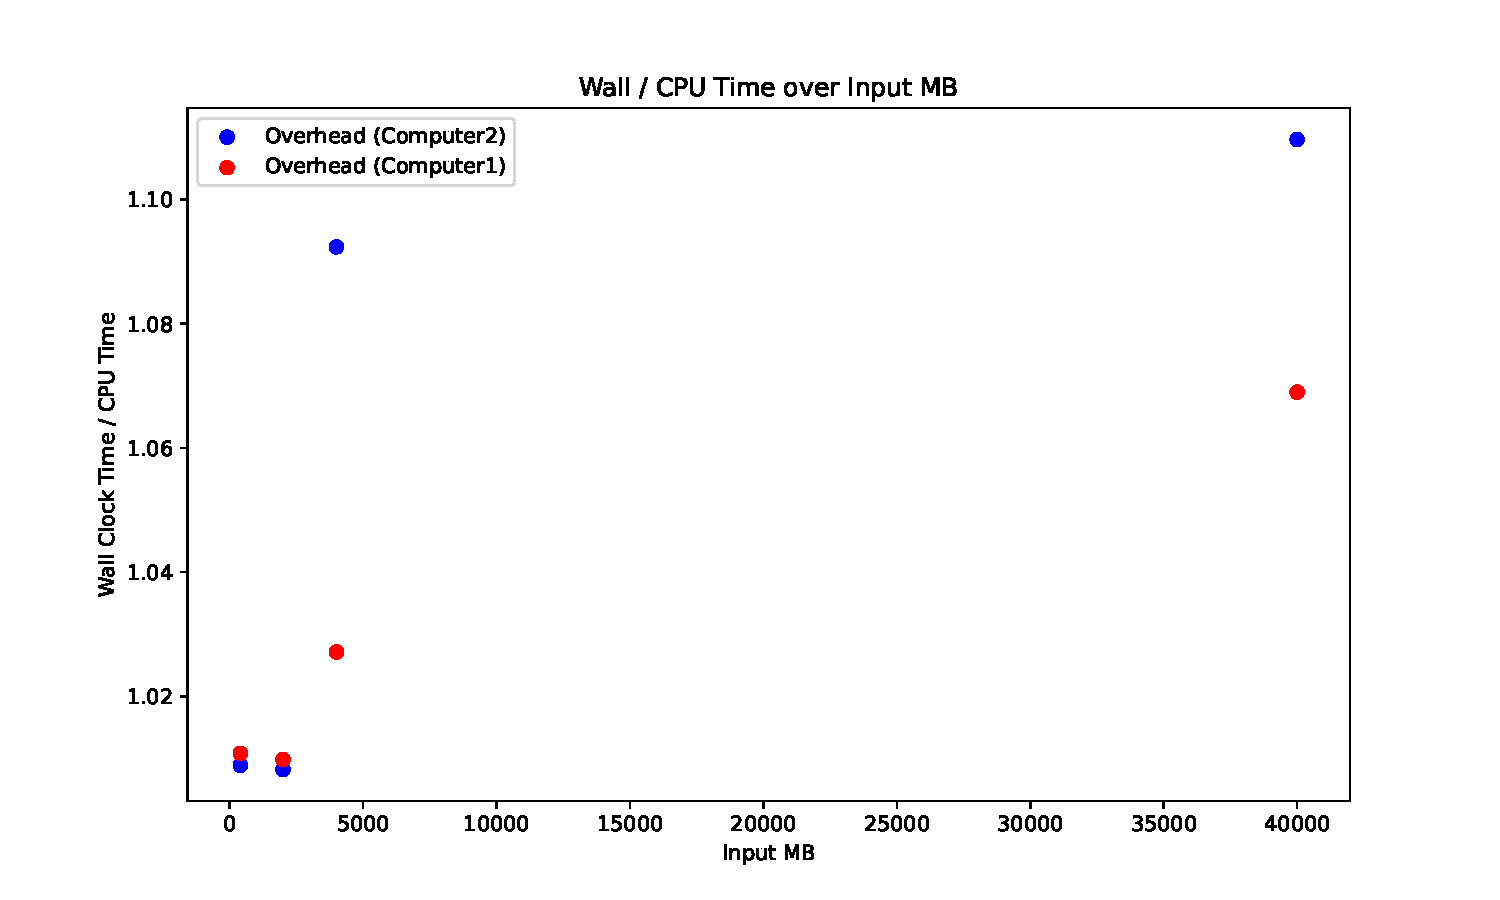
\includegraphics[width=\textwidth]{./res/overhead_ratio.pdf}
        \caption{}
        \label{fig:overhead_ratio.pdf}
    \end{minipage}
\end{figure}
% TODO

\paragraph*{Optimizing Performance with a Fast In-Place Sorting Algorithm}
We can outperform Classical Merge Sort on some instances by using Quick Sort for the internal sorting and provide statistical evidence below.
We will show that External Memory Merge Sort with Quick Sort for the in-place sorting < Classical Merge Sort < External Memory Merge Sort with Classical Merge Sort for the in-place sorting.
% TODO

\paragraph*{Optimizing Performance with a Large Block Size}
We want to do as little I/O operations as possible, due to their slowness. Since External Memory Merge Sort is supposed to be applied to data sets larger than the available internal memory,
we have to accept the cost of I/O operations at some point. Nevertheless, large block sizes allow for less I/O operations. In the inital partitioning phase, we benefit from internal sortation
in greater proportion relative to I/O operations and we need less merge rounds in the following merging phase.
The evidence from experiments is shown below.
% TODO

\paragraph*{Optimizing Performance with a Binary Comparison Function}
We will see if choosing a comparison function fit for the binary format of the input data can outperform a naive implementation of the comparison function that Quick Sort uses
in the External Memory Merge Sort in-place sorting phase.
% TODO

\paragraph*{Optimizing Performance with Better Compiler Optimizations}
We will see if an enhanced compiler optimization strategy improves the run times.
gcc -O3 vs gcc -O3 -marchnative...
% TODO

\paragraph*{Optimizing Performance by Changing the Computing Environment}
It is clear that the computing environment must have an influence on the performance.
We observe significant differences of run times between different computing environments.
% Additionally, we use different computers to hedge our findings against random influences specific to a computer
% TODO

\paragraph*{Optimizing Performance with Block Size Multiples Relative to Underlying Storage Block Size}
\label{par:storage_block_size}
Factors such as storage block size, data distribution, and access patterns can significantly impact the optimal block size for a given scenario.
It is essential to consider the interplay between these variables to make informed decisions about block size selection and achieve optimal performance.
While larger block sizes generally enhance overall system performance, it is important to note that this principle does not directly apply on a small scale.
To achieve maximum efficiency, it is crucial to align block sizes with multiples of the system's storage block size.
When we read consecutive blocks into the internal memory, a non-multiple block size necessitates accessing some elements from the last storage block of the
preceding read during the subsequent read operation.
This overlapping pattern persists until the accumulated overlap is vanishes because it becomes divisible by the storage block size.
One such access pattern is given below (Figure \ref{fig:access_pattern_decrement.pdf}). Along with it, we give an improved access pattern, where we visualize the advantage of selecting
a block size that is a multiple of the storage block size (Figure \ref{fig:improved_access_pattern.pdf}). We then show another access pattern with a bigger block size to demonstrate
this counter-intuitive local inefficiency for a block size increment (Figure \ref{fig:access_pattern_increment.pdf}). Each time, the diagrams show the actions to load \( 4 \) blocks of block size
into our internal memory.
This is because the system's storage block size represents the smallest unit of data that can be loaded into the internal memory.

In a nuanced analysis of the anticipated number of read operations, we can delineate the expected efficiencies of various block sizes (Figure \ref{fig:expected_io_performance_analysis.pdf}).
Thereat, we establish a connection to the greatest common divisor of the storage block size and the block size (Figure \ref{fig:gcd_vs_io_performance_analysis.pdf}).
This factor significantly influences the local performance of different block sizes.

\begin{figure}[htb]
    \begin{minipage}{0.475 \textwidth}
        \centering
        \includegraphics[width=0.8 \textwidth]{./res/gcd_multiples_efficiency/access_pattern_decrement.pdf}
        \caption{A possible access pattern when we assume a storage block size of \( 4 \) and a block size of \( 7 \) to read from the storage (green) into the internal memory (gold).
            We get \( 7 \) distinct storage blocks for \( 10 \) system reads. }
        \label{fig:access_pattern_decrement.pdf}
    \end{minipage}
\end{figure}

\begin{figure}[htb]
    \begin{minipage}{0.475 \textwidth}
        \centering
        \includegraphics[width=0.8 \textwidth]{./res/gcd_multiples_efficiency/improved_access_pattern.pdf}
        \caption{An improved access pattern for the storage block size of \( 4 \) with a block size of \( 8 \) to read from the storage (green) into the internal memory (gold).
            We get \( 8 \) distinct storage blocks for \( 8 \) system reads. }
        \label{fig:improved_access_pattern.pdf}
    \end{minipage}
\end{figure}

\begin{figure}[htb]
    \begin{minipage}{0.475 \textwidth}
        \centering
        \includegraphics[width=0.8 \textwidth]{./res/gcd_multiples_efficiency/access_pattern_increment.pdf}
        \caption{A possible access pattern when we assume a storage block size of \( 4 \) and a block size of \( 9 \) to read from the storage (green) into the internal memory (gold).
            We get \( 9 \) distinct storage blocks for \( 12 \) system reads. }
        \label{fig:access_pattern_increment.pdf}
    \end{minipage}
\end{figure}

\begin{figure}[htb]
    \begin{minipage}{0.475 \textwidth}
        \centering
        \includegraphics[width=0.8 \textwidth]{./res/gcd_multiples_efficiency/expected_io_performance_analysis.pdf}
        \caption{Analysis on the expected read efficiency due to access patterns and divisibility of block sizes. We measure read efficiency in Distinct Storage Blocks Read\( / \)Storage Blocks Read. }
        \label{fig:expected_io_performance_analysis.pdf}
    \end{minipage}
\end{figure}

\begin{figure}[htb]
    \begin{minipage}{0.475 \textwidth}
        \centering
        \includegraphics[width=0.8 \textwidth]{./res/gcd_multiples_efficiency/gcd_vs_io_performance_analysis.pdf}
        \caption{Analysis on the expected read efficiency due to access patterns and divisibility of block sizes. We measure read efficiency in Distinct Storage Blocks Read\( / \)Storage Blocks Read and
            GCD efficiency in GCD(Storage Block Size, Block Size)\( / \)Storage Block Size. Favorable block sizes have efficiency peaks where the GCD efficiency is high. }
        \label{fig:gcd_vs_io_performance_analysis.pdf}
    \end{minipage}
\end{figure}

\begin{figure}[htb]
    \begin{minipage}{0.475 \textwidth}
        \centering
        \includegraphics[width=0.8 \textwidth]{./res/gcd_multiples_efficiency/limited_expected_io_performance_analysis.pdf}
        \caption{Analysis on the expected read efficiency due to access patterns and divisibility of block sizes. We measure read efficiency in Distinct Storage Blocks Read\( / \)Storage Blocks Read. Demonstration of
            counter-intuitive local efficiencies around the block size value \( 4 \times 4096 = 16\,384 \) due to access patterns that are to be expected. }
        \label{fig:limited_expected_io_performance_analysis.pdf}
    \end{minipage}
\end{figure}

We can see that for the External Memory Merge Sort algorithm, the median run time is lower with the block size selected as a multiple of the system's storage block size
(Figure \ref{fig:visualization_multiples_block_size.png}).
The distribution shift that results from the different block sizes is visualized with kernel density estimations (KDE) (Figure \ref{fig:kde_plot_multiples_block_size.png}).
\begin{figure*}
    \centering
    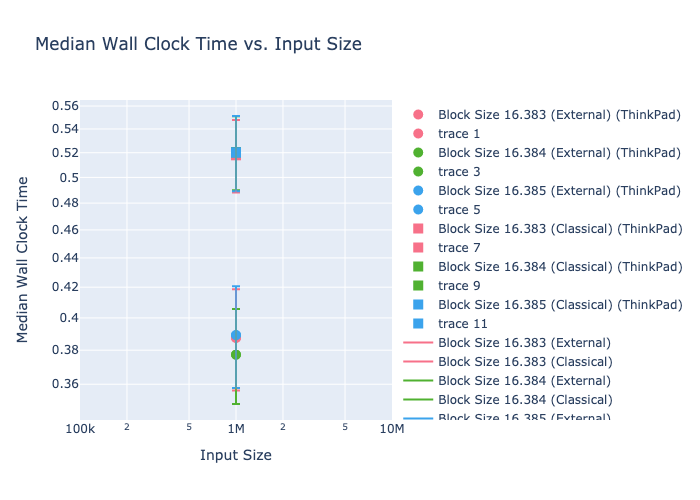
\includegraphics[width=0.8 \textwidth]{./res/visualization_multiples_block_size.png}
    \caption{Boxplots with medians and inter-quartile ranges for the distributions of \( 40 \) runs on \( 100 \) files with the block sizes \( 16\,383, 16\,384 \) and \( 16\,385\) (\(4\,096\) is
        the underlying storage block size).}
    \label{fig:visualization_multiples_block_size.png}
\end{figure*}
\begin{figure*}
    \centering
    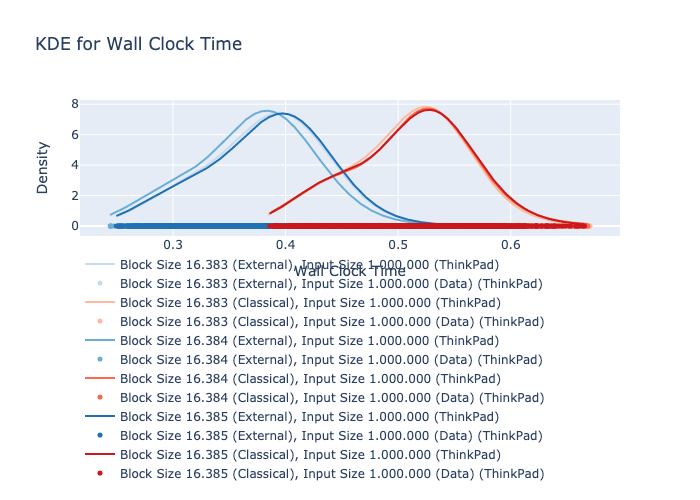
\includegraphics[width=0.8 \textwidth]{./res/kde_plot_multiples_block_size.png}
    \caption{Kernel density estimation plot for the distributions from \( 40 \) runs on \( 100 \) files with the block sizes \( 16\,383, 16\,384 \) and \( 16\,385 \) (\(4\,096\) is the underlying storage block size and
        \( 16\,384 = 4\,096 \times 4 \)). External Sorting (blue) uses Quick Sort for in-place sorting and is faster than Classical Sorting (red). A block size parameter set to a multiple of the underlying operating system's storage block size enhances performance significantly with a small effect size when compared to its decrement or increment (Paragraph \ref{par:storage_block_size}).}
    \label{fig:kde_plot_multiples_block_size.png}
\end{figure*}

To solidify our understanding of this behaviour, we do hypothesis tests (\( t \)-tests) regarding block size comparisons and report the \( p \)-value to determine significance and Cohen's \( d \) for the effect size.
We can deviate from the data normality assumption since we have large samples sizes.
With \( 40 \) runs on \( 100 \) random files, these are (\(40 > 30 \)) for each file, and (\(4\,000 > 30 \)) for the global analyses.
According to the Central Limit Theorem, even if the underlying data is not normally distributed, the distribution of sample means will tend to be approximately normal, hence the
distribution of differences of sample means will follow a \( t \) distribution.
Additionally, we can assume that any two run times are independent of each other, signifying the absence of any "lasting effects" from one run on ensuing ones.
Furthermore, we assume that the variances of the data are approximately equal. From the hypothesis tests, we get that choosing the block size as a multiple of the underlying sytem's storage blocksize
has a small (Cohen's \( d \approx 0.02 \)) beneficial effect compared to choosing the block size as one decrement or increment from the multiple.

\begin{figure}[htb]
    \begin{minipage}{0.475 \textwidth}
        \centering
        \includegraphics[width=\linewidth]{./res/multiples_hypothesis_test_results/KDE_for_Cohen's_d_of_Classical_Wall_Clock_Time.pdf}
        \caption{Cohen's \(d\) has less variance around zero indicating smaller effects of the block size on the algorithm performance (as it should be since Classical Merge Sort does not use the block size parameter)
            (Figure \ref{fig:KDE_for_Cohen's_d_of_External_Wall_Clock_Time.pdf}).}
        \label{fig:KDE_for_Cohen's_d_of_Classical_Wall_Clock_Time.pdf}
    \end{minipage}
\end{figure}

\begin{figure}[htb]
    \begin{minipage}{0.475 \textwidth}
        \centering
        \includegraphics[width=\linewidth]{./res/multiples_hypothesis_test_results/KDE_for_Cohen's_d_of_External_Wall_Clock_Time.pdf}
        \caption{Cohen's \(d\) has greater variance around zero indicating greater effects of the block size on the algorithm performance (as it should be since
            External Memory Merge Sort depends on the block size parameter)
            (Figure \ref{fig:KDE_for_Cohen's_d_of_Classical_Wall_Clock_Time.pdf}).}
        \label{fig:KDE_for_Cohen's_d_of_External_Wall_Clock_Time.pdf}
    \end{minipage}
\end{figure}

\begin{figure}[htb]
    \begin{minipage}{0.475 \textwidth}
        \centering
        \includegraphics[width=\linewidth]{./res/multiples_hypothesis_test_results/KDE_for_Cohen's_d_values_of_External_Wall_Clock_Time_(Block_Size_16383_vs_16384).pdf}
        \caption{Cohen's \(d\) is concentrated around the value \( 0.2 \), indicating a small positive effect of choosing the storage blocksize multiple as a blocksize over its decrement.}
        \label{fig:KDE_for_Cohen's_d_values_of_External_Wall_Clock_Time_(Block_Size_16383_vs_16384).pdf}
    \end{minipage}
\end{figure}

\begin{figure}[htb]
    \begin{minipage}{0.475 \textwidth}
        \centering
        \includegraphics[width=\linewidth]{./res/multiples_hypothesis_test_results/KDE_for_Cohen's_d_values_of_External_Wall_Clock_Time_(Block_Size_16383_vs_16385).pdf}
        \caption{Cohen's \(d\) is concentrated around zero, indicating no significant difference of choosing the decrement of the storage blocksize multiple versus the increment.}
        \label{fig:KDE_for_Cohen's_d_values_of_External_Wall_Clock_Time_(Block_Size_16383_vs_16385).pdf}
    \end{minipage}
\end{figure}

\begin{figure}[htb]
    \begin{minipage}{0.475 \textwidth}
        \centering
        \includegraphics[width=\linewidth]{./res/multiples_hypothesis_test_results/KDE_for_Cohen's_d_values_of_External_Wall_Clock_Time_(Block_Size_16384_vs_16385).pdf}
        \caption{Cohen's \(d\) is concentrated around the value \( -0.5 \) and the "global" hypothesis test's Cohen's d value for this setting is around \( -0.2 \),
            indicating a small negative effect of choosing the increment of a storage blocksize multiple over the multiple.}
        \label{fig:KDE_for_Cohen's_d_values_of_External_Wall_Clock_Time_(Block_Size_16384_vs_16385).pdf}
    \end{minipage}
\end{figure}

\begin{figure}[htb]
    \begin{minipage}{0.475 \textwidth}
        \centering
        \includegraphics[width=\linewidth]{./res/multiples_hypothesis_test_results/KDE_for_p-values_of_Classical_Wall_Clock_Time_(Block_Size_16383_vs_16384).pdf}
        \caption{The distribution of \( p \)-values looks similar for different block size comparisons. This is expected behaviour since the block sizes should not influence the run times for the Classical Merge
            Sort algorithm. With External Memory Merge Sort, we reject more often in the decrement vs. muliple case (Figure \ref{fig:KDE_for_p-values_of_External_Wall_Clock_Time_(Block_Size_16383_vs_16384).pdf}).}
        \label{fig:KDE_for_p-values_of_Classical_Wall_Clock_Time_(Block_Size_16383_vs_16384).pdf}
    \end{minipage}
\end{figure}

\begin{figure}[htb]
    \begin{minipage}{0.475 \textwidth}
        \centering
        \includegraphics[width=\linewidth]{./res/multiples_hypothesis_test_results/KDE_for_p-values_of_External_Wall_Clock_Time_(Block_Size_16383_vs_16384).pdf}
        \caption{The distribution of \( p \)-values for External Merge Sort for a storage block size multiple and its decrement shows an increase in \( p \)-values smaller than
            our significance level \( \alpha = 0.05 \). This illustrates that we reject similarity more often than with Classical Merge Sort in this setting
            (Figure \ref{fig:KDE_for_p-values_of_Classical_Wall_Clock_Time_(Block_Size_16383_vs_16384).pdf}).}
        \label{fig:KDE_for_p-values_of_External_Wall_Clock_Time_(Block_Size_16383_vs_16384).pdf}
    \end{minipage}
\end{figure}

\begin{figure}[htb]
    \begin{minipage}{0.475 \textwidth}
        \centering
        \includegraphics[width=\linewidth]{./res/multiples_hypothesis_test_results/KDE_for_p-values_of_Classical_Wall_Clock_Time_(Block_Size_16383_vs_16385).pdf}
        \caption{The distribution of \( p \)-values looks similar for different block size comparisons. This is expected behaviour since the block sizes should not influence the run times for the Classical Merge
            Sort algorithm. For this decrement vs. increment setting, similarity of run times are also not rejected with the External Memory Merge Sort algorithm
            (Figure \ref{fig:KDE_for_p-values_of_External_Wall_Clock_Time_(Block_Size_16383_vs_16385).pdf}).}
        \label{fig:KDE_for_p-values_of_Classical_Wall_Clock_Time_(Block_Size_16383_vs_16385).pdf}
    \end{minipage}
\end{figure}

\begin{figure}[htb]
    \begin{minipage}{0.475 \textwidth}
        \centering
        \includegraphics[width=\linewidth]{./res/multiples_hypothesis_test_results/KDE_for_p-values_of_External_Wall_Clock_Time_(Block_Size_16383_vs_16385).pdf}
        \caption{The distribution of \( p \)-values for External Merge Sort for the decrement and the increment of a storage block size multiple does not have a large increase in \( p \)-values
            smaller than our significance level \( \alpha = 0.05 \). This illustrates that we do not reject similarity more often than in our Classical Merge Sort neutral "base case", indicating similarity of the samples' underlying population means.
            (Figure \ref{fig:KDE_for_p-values_of_Classical_Wall_Clock_Time_(Block_Size_16383_vs_16385).pdf}).}
        \label{fig:KDE_for_p-values_of_External_Wall_Clock_Time_(Block_Size_16383_vs_16385).pdf}
    \end{minipage}
\end{figure}

\begin{figure}[htb]
    \begin{minipage}{0.475 \textwidth}
        \centering
        \includegraphics[width=\linewidth]{./res/multiples_hypothesis_test_results/KDE_for_p-values_of_Classical_Wall_Clock_Time_(Block_Size_16384_vs_16385).pdf}
        \caption{The distribution of \( p \)-values looks similar for different block size comparisons. This is expected behaviour since the block sizes should not influence the run times for the Classical Merge
            Sort algorithm as opposed to the External Memory Merge Sort algorithm (Figure \ref{fig:KDE_for_p-values_of_External_Wall_Clock_Time_(Block_Size_16384_vs_16385).pdf}).}
        \label{fig:KDE_for_p-values_of_Classical_Wall_Clock_Time_(Block_Size_16384_vs_16385).pdf}
    \end{minipage}
\end{figure}

\begin{figure}[htb]
    \begin{minipage}{0.475 \textwidth}
        \centering
        \includegraphics[width=\linewidth]{./res/multiples_hypothesis_test_results/KDE_for_p-values_of_External_Wall_Clock_Time_(Block_Size_16384_vs_16385).pdf}
        \caption{The distribution of \( p \)-values for External Merge Sort for a storage block size multiple and its increment shows an increase in \( p \)-values smaller
            than our significance level \( \alpha = 0.05 \). This illustrates that we reject similarity more often in this setting than with Classical Merge Sort (Figure \ref{fig:KDE_for_p-values_of_Classical_Wall_Clock_Time_(Block_Size_16384_vs_16385).pdf}).}
        \label{fig:KDE_for_p-values_of_External_Wall_Clock_Time_(Block_Size_16384_vs_16385).pdf}
    \end{minipage}
\end{figure}

\begin{figure}[htb]
    \begin{minipage}{0.475 \textwidth}
        \centering
        \includegraphics[width=\linewidth]{./res/multiples_hypothesis_test_results/KDE_for_p-values_of_Classical_Wall_Clock_Time.pdf}
        \caption{The distribution of \( p \)-values for the Classical Merge Sort algorithm has less \( p \)-values below our significance level \( \alpha = 0.05 \) than in the External Memory Merge Sort case (Figure \ref{fig:KDE_for_p-values_of_External_Wall_Clock_Time.pdf}).}
        \label{fig:KDE_for_p-values_of_Classical_Wall_Clock_Time.pdf}
    \end{minipage}
\end{figure}

\begin{figure}[htb]
    \begin{minipage}{0.475 \textwidth}
        \centering
        \includegraphics[width=\linewidth]{./res/multiples_hypothesis_test_results/KDE_for_p-values_of_External_Wall_Clock_Time.pdf}
        \caption{The distribution of \( p \)-values for External Merge Sort displays more \( p \)-values below our significance level \( \alpha = 0.05 \) than in the Classical Merge Sort case (Figure \ref{fig:KDE_for_p-values_of_Classical_Wall_Clock_Time.pdf}).}
        \label{fig:KDE_for_p-values_of_External_Wall_Clock_Time.pdf}
    \end{minipage}
\end{figure}

\begin{figure}[htb]
    \begin{minipage}{0.475 \textwidth}
        \centering
        \includegraphics[width=\linewidth]{./res/multiples_hypothesis_test_results/T-test_Results_for_Classical_Wall_Clock_Time_(Block_Size_16383_vs_16384).pdf}
        \caption{Comparison of "Reject" vs. "Fail to Reject" decisions as hypothesis test results from \( 100 \) hypothesis tests with \( 40 \) measurements for each test.
            In Classical Merge Sort, we reject less often than in External Memory Merge Sort (Figure \ref{fig:T-test_Results_for_External_Wall_Clock_Time_(Block_Size_16383_vs_16384).pdf}).
            We attribute the variation between the block size comparisons to random influences as Classical Merge Sort does not take a block size as an algorithm parameter.}
        \label{fig:T-test_Results_for_Classical_Wall_Clock_Time_(Block_Size_16383_vs_16384).pdf}
    \end{minipage}
\end{figure}

\begin{figure}[htb]
    \begin{minipage}{0.475 \textwidth}
        \centering
        \includegraphics[width=\linewidth]{./res/multiples_hypothesis_test_results/T-test_Results_for_External_Wall_Clock_Time_(Block_Size_16383_vs_16384).pdf}
        \caption{With External Memory Merge Sort we reject more than with Classical Merge Sort considering the block size comparison between the decrement and the multiple (Figure \ref{fig:T-test_Results_for_Classical_Wall_Clock_Time_(Block_Size_16383_vs_16384).pdf}).}
        \label{fig:T-test_Results_for_External_Wall_Clock_Time_(Block_Size_16383_vs_16384).pdf}
    \end{minipage}
\end{figure}

\begin{figure}[htb]
    \begin{minipage}{0.475 \textwidth}
        \centering
        \includegraphics[width=\linewidth]{./res/multiples_hypothesis_test_results/T-test_Results_for_Classical_Wall_Clock_Time_(Block_Size_16383_vs_16385).pdf}
        \caption{Comparison of "Reject" vs. "Fail to Reject" decisions as hypothesis test results from \( 100 \) hypothesis tests with \( 40 \) measurements for each test.
            In Classical Merge Sort, we reject less often than in External Memory Merge Sort (Figure \ref{fig:T-test_Results_for_External_Wall_Clock_Time_(Block_Size_16383_vs_16385).pdf}).
            We attribute the variation between the block size comparisons to random influences as Classical Merge Sort does not take a block size as an algorithm parameter.}
        \label{fig:T-test_Results_for_Classical_Wall_Clock_Time_(Block_Size_16383_vs_16385).pdf}
    \end{minipage}
\end{figure}

\begin{figure}[htb]
    \begin{minipage}{0.475 \textwidth}
        \centering
        \includegraphics[width=\linewidth]{./res/multiples_hypothesis_test_results/T-test_Results_for_External_Wall_Clock_Time_(Block_Size_16383_vs_16385).pdf}
        \caption{For the increment versus decrement block size comparison, we reject about as often as with Classical Merge Sort (Figure \ref{fig:T-test_Results_for_Classical_Wall_Clock_Time_(Block_Size_16383_vs_16385).pdf}). This indicates the absence of a significant difference in run times for these two block sizes.}
        \label{fig:T-test_Results_for_External_Wall_Clock_Time_(Block_Size_16383_vs_16385).pdf}
    \end{minipage}
\end{figure}

\begin{figure}[htb]
    \begin{minipage}{0.475 \textwidth}
        \centering
        \includegraphics[width=\linewidth]{./res/multiples_hypothesis_test_results/T-test_Results_for_Classical_Wall_Clock_Time_(Block_Size_16384_vs_16385).pdf}
        \caption{Comparison of "Reject" vs. "Fail to Reject" decisions as hypothesis test results from \( 100 \) hypothesis tests with \( 40 \) measurements for each test.
            In Classical Merge Sort, we reject less often than in External Memory Merge Sort (Figure \ref{fig:T-test_Results_for_External_Wall_Clock_Time_(Block_Size_16384_vs_16385).pdf}).
            We attribute the variation between the block size comparisons to random influences as Classical Merge Sort does not take a block size as an algorithm parameter.}
        \label{fig:T-test_Results_for_Classical_Wall_Clock_Time_(Block_Size_16384_vs_16385).pdf}
    \end{minipage}
\end{figure}

\begin{figure}[htb]
    \begin{minipage}{0.475 \textwidth}
        \centering
        \includegraphics[width=\linewidth]{./res/multiples_hypothesis_test_results/T-test_Results_for_External_Wall_Clock_Time_(Block_Size_16384_vs_16385).pdf}
        \caption{For the storage multiple versus its increment, we see again that we reject more often than with Classical Merge Sort (which acts as the "neutral base case" here) (Figure \ref{fig:T-test_Results_for_Classical_Wall_Clock_Time_(Block_Size_16384_vs_16385).pdf}).}
        \label{fig:T-test_Results_for_External_Wall_Clock_Time_(Block_Size_16384_vs_16385).pdf}
    \end{minipage}
\end{figure}

\begin{figure}[htb]
    \begin{minipage}{0.475 \textwidth}
        \centering
        \includegraphics[width=\linewidth]{./res/multiples_hypothesis_test_results/T-test_Results_for_Classical_Wall_Clock_Time_(Global).pdf}
        \caption{Aggregated comparison of "Reject" vs. "Fail to Reject" decisions as hypothesis test results from three different block sizes with each \( 100 \) hypothesis tests with \( 40 \) measurements for each test. In Classical Merge Sort, we reject less often than in External Memory Merge Sort (Figure \ref{fig:T-test_Results_for_External_Wall_Clock_Time_(Global).pdf}).
            We attribute the variation between the block size comparisons to random influences as Classical Merge Sort does not take a block size as an algorithm parameter.}
        \label{fig:T-test_Results_for_Classical_Wall_Clock_Time_(Global).pdf}
    \end{minipage}
\end{figure}

\begin{figure}[htb]
    \begin{minipage}{0.475 \textwidth}
        \centering
        \includegraphics[width=\linewidth]{./res/multiples_hypothesis_test_results/T-test_Results_for_External_Wall_Clock_Time_(Global).pdf}
        \caption{With External Memory Merge Sort, in total, we reject the similarity null hypothesis more often than with Classical Merge Sort (Figure \ref{fig:T-test_Results_for_Classical_Wall_Clock_Time_(Global).pdf}). This is indicative of the presence of an effect that the choice of the block sze parameter
            near a multiple of the underlying storage block size has on the performance of our External Memory Merge Sort algorithm.}
        \label{fig:T-test_Results_for_External_Wall_Clock_Time_(Global).pdf}
    \end{minipage}
\end{figure}

\begin{center}
    %\includegraphics[width=0.5\textwidth]{res/bar-graph}
\end{center}

For the Classical Merge Sort algorithm, an initial blocksize of \( 1 \) was assumed and for the external memory algorithm, the initial blocksize was set such that the size of blocks in use does not exceed RAM size.


\section{Discussion and Conclusion}
% In this section, the results are discussed and interpreted. Finally, the work is summarized shortly.

\paragraph{Areas of improvement}
Multi-way merging, that is, merging more than two blocks at the same time, with \( k > 2 \)  in the \( k \)-way merge, is anticipated to boost performance levels.
However, increasing \(k\) too much can lead to excessive memory usage and potentially degrade performance due to increased I/O operations.
Leveraging multithreading capabilities is likely to further enhance overall performance significantly.
Implementing double buffering is anticipated to alleviate I/O wait times and consequently enhance the overall runtime performance of the algorithm.
For the initial partitioning phase, it is possible to implement a parallel sorting algorithm to expedite the process.
In the subsequent phase, there is an opportunity to concurrently merge different segments or even initiate merging while I/O operations are still underway.

\paragraph{Conlusions}


\section{References}
Provided material and exercise sheet \( 1\) of the lecture "Algorithm Engineering, Winter 2023/24, University of Konstanz".

\end{document}
